\LectureAnswerSection\subsection*{两级提示}
\phantomsection\label{hint:at4:drill:1}
\LectureHint{at4:drill:1}{先把全部表达式写成无量纲小参数。}{最近距离的差与相对差分开比较。}
\phantomsection\label{hint:at4:drill:2}
\LectureHint{at4:drill:2}{转角随近点距离增大而减小。}{安全半径为正时检查反正弦的严格范围。}
\phantomsection\label{hint:at4:drill:3}
\LectureHint{at4:drill:3}{将两个恒星系动能展开，相同平方项相消。}{判断沿行星速度的投影是否增加。}
\phantomsection\label{hint:at4:drill:4}
\LectureHint{at4:drill:4}{相同速率和位置只保证相同能量。}{另算角动量，零值必须单独处理。}
\phantomsection\label{hint:at4:drill:5}
\LectureHint{at4:drill:5}{比较入射正能量与椭圆负能量。}{若能量交换存在，明确选取的系统边界。}
\phantomsection\label{hint:at4:drill:6}
\LectureHint{at4:drill:6}{偏转角阈值转成冲量参数上限。}{若只统计掠过，减去会撞入表面的中心截面。}
\phantomsection\label{hint:at4:drill:7}
\LectureHint{at4:drill:7}{先用短时动量关系。}{动能求微分时质量和速度都在变化。}
\phantomsection\label{hint:at4:drill:8}
\LectureHint{at4:drill:8}{能量差是行星速度与余速变化的点积。}{两等长速度矢量之差是速度圆的一条弦。}
\Needspace{8\baselineskip}\subsection*{详解}
\begin{drillsolution}{at4:drill:1}
图\ref{fig:at4:drill:1:s} 的精确关系是 $\chi=2\arctan\eta$，故 $\chi=2\eta+O(\eta^3)$。最近距离由 $r_p=(\mu/v_\infty^2)(\sqrt{1+\eta^{-2}}-1)$ 得
\[r_p=b\big(\sqrt{1+\eta^2}-\eta\big)=b(1-\eta)+O(b\eta^2).
\]
\typeout{ASTROFIG:fig:at4:drill:1:p}\fig{fig:at4:drill:1:p}{解答过程：弱偏转的最近距离修正}{\begin{tikzpicture}[scale=.85]
\draw[guide](-4.5,-1.1055)--(4.5,-1.1055);\draw[world,domain=-2:2,samples=100]plot({(.11111111*(10-cosh(\x))+9.94987437*1.1055416*sinh(\x))/10},{(-9.94987437*.11111111*(10-cosh(\x))+1.1055416*sinh(\x))/10});\fill(0,0)circle(2pt)node[above]{$F$};\draw[flow](-4.1,-1.1055)--(-3,-1.1055)node[below]{$v_\infty$};\node at(0,1){$r_p\simeq b-\mu/v_\infty^2$};
\end{tikzpicture}}

图\ref{fig:at4:drill:1:p} 中最近距离比冲量参数略小，差约 $\mu/v_\infty^2$。虽然绝对修正形式不含 $b$，其相对修正 $\eta$ 会随 $b$ 增大而变小；只有在 $\eta\ll1$ 下这个展开才成立。不能把角度的一阶近似与任意强引力近点同时使用。\end{drillsolution}
\begin{drillsolution}{at4:drill:2}
图\ref{fig:at4:drill:2:s} 有 $e=1+r_pu^2/\mu_p$，$\chi=2\arcsin(1/e)$ 随 $r_p$ 增大而减小。因此 图\ref{fig:at4:drill:2:p} 的最小允许近点给
\[\chi_{\max}=2\arcsin\frac1{1+r_{\min}u^2/\mu_p},\qquad
b_{\min}=r_{\min}\sqrt{1+\frac{2\mu_p}{r_{\min}u^2}}.
\]
\typeout{ASTROFIG:fig:at4:drill:2:p}\fig{fig:at4:drill:2:p}{解答过程：给定余速与安全半径的最大转角}{\begin{tikzpicture}[scale=.85]
\draw[guide](-4.6,-1.118)--(1,-1.118);\draw[world,domain=-2:2,samples=110]plot({(1.5-cosh(\x))/1.5+1.11803399*1.11803399*sinh(\x)/1.5},{-1.11803399*(1.5-cosh(\x))/1.5+1.11803399*sinh(\x)/1.5});\fill(0,0)circle(2pt)node[above left]{$F$};\draw[flow](-4.2,-1.118)--(-3,-1.118)node[midway,below]{$u$};\node at(-2,2){$r_p=r_{\min}$};\node at(-2,1.3){$\chi_{\max}<\pi$};
\end{tikzpicture}}

若 $r_{\min}>0,u>0$，反正弦的自变量严格小于一，转角严格小于 $\pi$，故不能精确180度反转。小余速可以使转角接近180度，却不能忽略对应的长接近时间、行星影响区和其他天体扰动。\end{drillsolution}
\begin{drillsolution}{at4:drill:3}
图\ref{fig:at4:drill:3:s} 的两种恒星系速度为 $\bm V+\bm u_{\rm in,out}$。近似在相同日心位置比较时，恒星势能相同，行星系的 $u^2/2$ 也相同，展开两动能之差得到
\[\Delta\varepsilon=\frac12\big(|\bm V+\bm u_{\rm out}|^2-|\bm V+\bm u_{\rm in}|^2\big)
=Vu(\cos\beta-\cos\alpha).
\]
\typeout{ASTROFIG:fig:at4:drill:3:p}\fig{fig:at4:drill:3:p}{解答过程：引力助推的能量正负}{\begin{tikzpicture}[scale=.85]
\draw[axis](0,0)--(4,0)node[right]{沿 $\bm V$ 的分量};\draw[flow](0,1)--(1.3,1)node[right]{$u\cos\alpha$};\draw[flow,blue](0,2)--(3,2)node[right]{$u\cos\beta$};
\end{tikzpicture}}

图\ref{fig:at4:drill:3:p} 的出射余速更朝向行星速度，即 $\cos\beta>\cos\alpha$，才给日心能量增加；反向绕过可能减速。由余弦范围有绝对上界 $|\Delta\varepsilon|\le2Vu$，但要达到该上界需180度转向，有限安全半径通常不允许。\end{drillsolution}
\begin{drillsolution}{at4:drill:4}
图\ref{fig:at4:drill:4:s} 两初态能量均为 $-\mu/(2r_0)$，所以有相同的有符号半长轴尺度 $r_0$。切向初态 $h=\sqrt{\mu r_0}$，得到 $e=0$，轨道为半径 $r_0$ 的圆。
\typeout{ASTROFIG:fig:at4:drill:4:p}\fig{fig:at4:drill:4:p}{解答过程：局部速度相同却有不同最近距离}{\begin{tikzpicture}[scale=.85]
\draw[world](0,0)circle(1.7);\draw[guide](0,0)--(3.4,0);\fill(3.4,0)circle(2pt)node[right]{$2r_0$};\node at(0,2.3){圆：$r=r_0$};\node at(2.4,-.8){径向：$r_{\max}=2r_0$};
\end{tikzpicture}}

图\ref{fig:at4:drill:4:p} 径向初态 $h=0$，是退化径向轨道，最高距离由 $-\mu/r_{\max}=-\mu/(2r_0)$ 给 $2r_0$，随后掉回中心或实际表面。可把点质点数学极限下的最近距离记零，但遇到实体表面就应停止延伸。相同机械能只固定轨道大小尺度，角动量还决定形状和可达边界。\end{drillsolution}
\begin{drillsolution}{at4:drill:5}
  图\ref{fig:at4:drill:5:s} 初始单位质量相对能量 $\varepsilon=v_\infty^2/2>0$，保守固定中心场中它始终不变。图\ref{fig:at4:drill:5:p} 的轨道虽然改变方向，远处速率仍为 $v_\infty$，故不能自动成为负能量椭圆。
  \typeout{ASTROFIG:fig:at4:drill:5:p}\fig{fig:at4:drill:5:p}{解答过程：无耗散引力能否自动捕获}{\begin{tikzpicture}[scale=.85]
\draw[flow](0,0)--(4,0);\node[above]at(0,0){$\varepsilon>0$ 入射};\node[above]at(4,0){$\varepsilon>0$ 出射};\node at(2,-1){无耗散二体不能自动转为负能量};
\end{tikzpicture}}

  若增加阻力、逆行点火或非弹性碰撞，探测器自身的机械能可以下降；若行星本身移动并与另一天体共同作用，应在完整系统中追踪能量交换。总能量守恒没有失效，但“探测器相对某一固定中心的二体能量”未必仍守恒。不同情形改变的是可使用的守恒量与系统边界。\end{drillsolution}
\begin{drillsolution}{at4:drill:6}
  图\ref{fig:at4:drill:6:s} 由 $\tan(\chi/2)=\mu/(bu^2)$，偏转角随 $b$ 增大而减小。因此 $\chi\ge\chi_0$ 要求 $0\le b\le b_0=\mu/[u^2\tan(\chi_0/2)]$。
  \typeout{ASTROFIG:fig:at4:drill:6:p}\fig{fig:at4:drill:6:p}{解答过程：超过给定偏转角的散射截面}{\begin{tikzpicture}[scale=.85]
\draw[world](0,0)circle(1.8);\draw[fill=gray!20](0,0)circle(.9);\node at(0,0){碰撞区};\node at(1.2,1){散射环};\node at(2.8,-.4){外半径 $b_0$};
\end{tikzpicture}}

  图\ref{fig:at4:drill:6:p} 点质量几何截面为 $\sigma=\pi b_0^2$。若有吸收半径 $R$，非碰撞轨道还需 $b>b_c=R\sqrt{1+2\mu/(Ru^2)}$。同时满足的大角无碰撞截面为 $\pi\max(0,b_0^2-b_c^2)$；边界是否允许相切不影响连续截面的面积值。不能把会撞入中心体的强偏转轨道同时计入“无碰撞散射”。\end{drillsolution}
\begin{drillsolution}{at4:drill:7}
  图\ref{fig:at4:drill:7:s} 初动量 $MV$，末动量 $(M+\dd M)(V+\dd V)$。保留一阶得 $M\dd V+V\dd M=0$，故 $\dd V=-V\dd M/M$。
  \typeout{ASTROFIG:fig:at4:drill:7:p}\fig{fig:at4:drill:7:p}{解答过程：吸收静止尘埃后的减速与耗散}{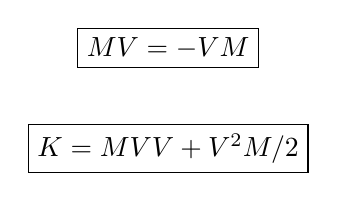
\begin{tikzpicture}[scale=.85]
\node[draw]at(0,1){$M\dd V=-V\dd M$};\node[draw]at(0,-.5){$\dd K=MV\dd V+V^2\dd M/2$};
\end{tikzpicture}}

  图\ref{fig:at4:drill:7:p} 末动能展开为 $MV^2/2+MV\dd V+V^2\dd M/2$，代入上式后，动能变化为 $-V^2\dd M/2$。因此不可逆机械能损失为 $V^2\dd M/2$，转入内能、形变等。仅计算 $MV\dd V$ 会多算一倍损失，漏掉质量增加本身携带的动能项。若把远处引力聚焦也包含在系统内，还须一致追踪势能与内能。\end{drillsolution}
\begin{drillsolution}{at4:drill:8}
  图\ref{fig:at4:drill:8:s} 两余速大小相同，$\Delta\varepsilon=\bm V\cdot(\bm u_{\rm out}-\bm u_{\rm in})$，因此柯西不等式给 $|\Delta\varepsilon|\le V|\Delta\bm u|$。
  \typeout{ASTROFIG:fig:at4:drill:8:p}\fig{fig:at4:drill:8:p}{解答过程：恒星系助推能量的上界为何不能随意取得}{\begin{tikzpicture}[scale=.85]
\draw[guide](0,0)circle(1.6);\draw[flow](0,0)--(1.6,0);\draw[flow,blue](0,0)--(-.8,1.386);\draw[force](1.6,0)--(-.8,1.386)node[midway,above]{$|\Delta\bm u|$};
\end{tikzpicture}}

  图\ref{fig:at4:drill:8:p} 速度圆上的弦长 $|\Delta\bm u|=2u\sin(\delta/2)$，所以
  \[|\Delta\varepsilon|\le2Vu\sin(\delta_{\max}/2)\le2Vu.
  \]
  前一个界要取得还需速度变化方向与 $\bm V$ 平行；若入射方向已经固定，也未必能达到。安全近点给 $\delta_{\max}<\pi$ 时，后一较宽上界严格不可达。上界用于排除不可能方案，不应在未检查几何条件时直接当作实际能量收益。\end{drillsolution}
